\documentclass[12pt]{article}
\linespread{1.6}

\usepackage{amsfonts}
\usepackage{amsmath}
\usepackage{amssymb}
\usepackage{caption}
\usepackage{cite}
\usepackage{float}
\usepackage{graphicx}
\usepackage{indentfirst}
\usepackage{lipsum}
\usepackage{multirow}
\usepackage{subcaption}
\usepackage{subfiles}
\usepackage{url}

\usepackage[T1]{fontenc}
\usepackage[utf8]{inputenc}
\usepackage[ddmmyyyy]{datetime}
\usepackage[english]{babel}
\usepackage[numbers]{natbib}
\usepackage[colorinlistoftodos,prependcaption]{todonotes}

% \setlength{\marginparwidth}{2cm}
% \usepackage{setspace}
% \onehalfspacing

\addtolength{\oddsidemargin}{-.5in}
\addtolength{\evensidemargin}{-.5in}
\addtolength{\textwidth}{1in}

\addtolength{\topmargin}{-.5in}
\addtolength{\textheight}{1in}

\renewcommand*\contentsname{Contents}
\renewcommand{\listfigurename}{List of Figures}
\renewcommand{\listtablename}{List of Tabelas}
\renewcommand*{\figurename}{Figure}
\renewcommand*{\tablename}{Table}
\renewcommand{\refname}{References}

\captionsetup{labelfont=bf}
\captionsetup{font=scriptsize}
%\newcommand{\figurescale}{0.7}

\begin{document}

\begin{figure}[t]
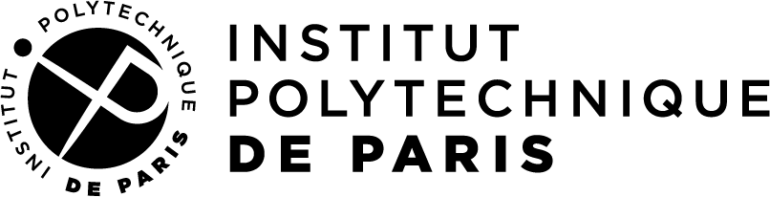
\includegraphics[width=0.7\columnwidth]{../figures/ipparis-logo.png}
\centering
\end{figure}

\begin{titlepage}
\begin{center}
Institut Polytechnique de Paris \\
Master IREN - Network Industries and Digital Economy \\
\vspace{44pt}

\huge Nested Syndication Networks: Community Structure and Hierarchical Organization in Innovation Ecosystems\\
\vspace{44pt}

\normalsize
\text{Master Thesis in Innovation Economy}\\  
\vspace{74pt}

\begin{center}
    \text{Authored by João Melga}\\ 
    \text{Advised by Jean-Michel Dalle}\\   
\end{center}

\vspace{\fill}
\today \\
\end{center}
\end{titlepage}

\pagenumbering{gobble}

\pagebreak

\section*{Abstract}

This study analyzes venture capital syndication networks using network theory to understand how investors organize and collaborate in funding startups. We examine 104,618 investment records from Crunchbase involving 38,843 investors and 16,932 companies to identify structural patterns in investor communities.

Using greedy modularity optimization, we discovered 170 distinct investor communities, with three large communities containing over 12,000 investors (75\% of the network). These communities exhibit power-law degree distributions typical of scale-free networks but differ significantly in investment activity and organization.

Our key finding is the emergence of significantly high nested structures within Community 2, which is dominated by Silicon Valley investors. This hierarchical organization enables substantially higher transaction volumes (33.6\% of all investments) compared to similarly-sized communities. The nested structure suggests that informal investment hierarchies systematically influence funding accessibility for entrepreneurs.

% Temporal analysis reveals that nestedness emerged through a sharp phase transition in 2019 rather than gradual evolution. This transition occurred when network connectance reached approximately 0.026, suggesting threshold-dependent emergence mechanisms. The pattern shows three phases: period with significantly low nestedness (2007-2018), rapid transition (2019), and sustained period with significantly high nestedness (2019-2024).

The concentration of nested structures specifically within Silicon Valley indicates that geographic clustering in innovation hubs may facilitate hierarchical investor relationships. High-degree investors in the nested community, particularly early-stage firms like SV Angel, function as network hubs that create efficient capital allocation pathways.

These findings challenge assumptions about random mixing in venture capital markets and suggest that network topology, rather than community size alone, determines investment ecosystem efficiency. The hierarchical organization may enhance stability against random investor departures but creates vulnerability to targeted removal of highly connected nodes.

Our results provide insights for ecosystem development strategies and suggest that understanding network structure is crucial for predicting investment patterns and improving access to capital for entrepreneurs.

\pagenumbering{gobble}
\pagebreak

\tableofcontents
\newpage

\pagenumbering{roman}
\setcounter{page}{1}

\addcontentsline{toc}{section}{List of Figures}
\listoffigures
\newpage

\addcontentsline{toc}{section}{List of Tables}
\listoftables
\newpage

\pagenumbering{arabic}
\setcounter{page}{1}

{
\setlength{\parskip}{0.7em}
\section*{Abstract}

\todo[inline]{To be done in the end}

\section{Introduction}

% -> Granoveter: To understand how people make economic decisions in the real world, you need to look at their social connections. We are neither isolated rational robots nor mere puppets of social norms. We are networks. And these networks shape our economic behaviors.

% - Talk about nestedness and bring concepts from "Nestedness in complex networks" for sure 

% - Talk about sindication

\todo[inline]{Improve introduction, it is still embrionary}

Two or more venture capital (VC) firms co-investing on the same enterprise is known in economics as syndication. In innovation networks, investors tend to behave like this so they can reduce the risk of investing in something not yet completelly validated or functional. In that case, reputation and centrality play an important role, once VCs will not only try to measure the potential return on investment (ROI), but also use its co-investors characteristics as a signal that interfers on their decisions.

The rising of syndicated investments in the last decades is evidence that innovation networks are by far a socialized network, where agents are not acting isolated, randomly, but in communities, being influenced by its peers. This phenomena is knwon as embededness.

Vast literature show how heavy tailled degree distributions emerge from such kind of interactions in social networks. In this same manner, innovation networks are not an exception, specially when it commes to number of connections of a certain player, as concentrated hubs of strongly connected agents can noramally be seen, while most part of the sample have only few ties, leading to a heterogenous distribtuion of connectance - also knwon as power-law degree distribution.

The widespread presence of power law degree distributions has incentivised numerous studies focused on uncovering plausible mechanisms behind their emergence, as well as exploring their impact on processes such as spreading dynamics \cite{PastorSatorras2001} and network robustness \cite{Albert2000}

When it comes to spreading dynamics, social and economic scientists have already explored how novel ideas are spread through networks, and how formation of bridge edges (with high betweeness) impact the chances of, for instance, novelty to spread in innovation networks. Well stablished ideas, like the Strengh of Weak Ties theory, are normally used as theoretical bases this kind of assumption.

In the other hand, measure the robustness to social and, being more specific, innnovation networks is still a theoretical and practical challenge. Impressivelly, ecology came to play an importat role to face it, and metrics like nestedness and the ecological consequences of its presence started to be transposed to social networks \cite{Theophile2024}.

On that paper, network theory is used to represent syndicated investments as edges of a network where investors are nodes with broad set of characteristics (geographic, financial, sectorial, etc.) This mathematical representation open horizions to better visualize and interpretate characteristics of this syndication network structure (or sub-networks inside of it) through ecology and economics lenses. 

Special attention is given for the fact that nestedness was observed among a certain group of early and late state investors.



\section{Methodology}

\subsection{Data Cleaning and Preprocessing}

This study uses data from Crunchbase, a commercial database that has emerged as a primary source for entrepreneurship and venture capital research \cite{OECD2017}. Founded in 2007 as a side project to TechCrunch, Crunchbase has evolved into a crowdsourced platform containing detailed information about startups, venture capital firms, accelerators, and investment rounds globally. The platform relies on multiple data collection methods, including user submissions, automated web crawling, partnerships with data providers, and editorial curation \cite{OECD2017}.

The dataset was obtained by querying Crunchbase for all investment transactions involving enterprises (startups, scale-ups, and growth companies) domiciled in the United States, which captures the complete investment ecosystem for US-based firms, including both domestic and cross-border capital flows. 

Foreign venture capital firms and institutional investors appear in the dataset when they participate in financing rounds of US enterprises. Furthermore, Crunchbase's coverage is particularly good for technology-oriented startups and venture capital transactions, making it well-suited for studies of innovation ecosystems and investment networks.

However, limitations and potential biases must be acknowledged when using Crunchbase data \cite{OECD2017}, for instance:

\begin{itemize}
    \item \textbf{Geographic bias}: Stronger coverage of US and Western European markets compared to emerging economies.
    \item \textbf{Sectoral bias}: Emphasis on technology and internet companies, potentially underrepresenting traditional industries.
    \item \textbf{Venture capital bias}: Better documentation of VC-backed companies compared to bootstrapped or debt-financed ventures (which may not be problematic for this study).
    \item \textbf{Size bias}: Larger and more successful companies are more likely to be thoroughly documented.
    \item \textbf{Temporal bias}: More recent information tends to be more complete and accurate than historical records.
\end{itemize}

These biases do not invalidate research using Crunchbase but require careful consideration in study design and interpretation of results. For network analysis of venture capital co-investments, the VC bias may actually enhance data quality by focusing on the target population of interest.

The data preprocessing and cleaning follows established methodologies from entrepreneurship literature \cite{Dalle2025} and is implemented through the following multi-step procedure:

\begin{enumerate}
    \item \textbf{Company data cleaning}: Removal of companies with incomplete essential information (missing unique identifiers, names, or founding years), exclusion of companies founded after 2017 to allow sufficient time for investment patterns to emerge, and removal of companies with exit status (closed, acquired, or IPO).
    
    \item \textbf{Investment data cleaning}: Removal of investment records with missing essential linkage information (company or investor identifiers), elimination of investments with invalid funding amounts (negative or zero values), and validation of funding consistency by excluding rounds where the sum of individual investments does not match the total funding amount reported in the database.
    
    \item \textbf{Funding threshold application}: Restriction of the sample to companies that raised more than \$150{,}000 in total funding to focus on substantive investment relationships and ensure stronger statistical reliability.
    
    % \item \textbf{Endogeneity bias prevention}: Exclusion of companies that received funding exclusively from accelerators or incubators to prevent endogeneity bias, as these companies may not have attracted independent market validation from external investors.
    
    \item \textbf{Data consistency validation}: Final consistency checks to ensure all investment records reference existing companies in the dataset and all retained companies have at least one valid investment record.
\end{enumerate}

\subsection{Network Construction}

The network construction process transforms raw investment data into a structured bipartite representation that enables theoretical reasoning about venture capital syndication patterns. This transformation follows the conceptual framework outlined by \cite{Borgatti2011}, who distinguish between flow models (focusing on how resources move through networks) and bond models (emphasizing coordination and solidarity among actors).

The construction process involves three sequential transformations, each representing a different conceptualization of network ties, each one described in \ref{fig:bipartite_pipeline} and in the subsequent paragraphs below.

\begin{figure}[htbp]
    \centering
    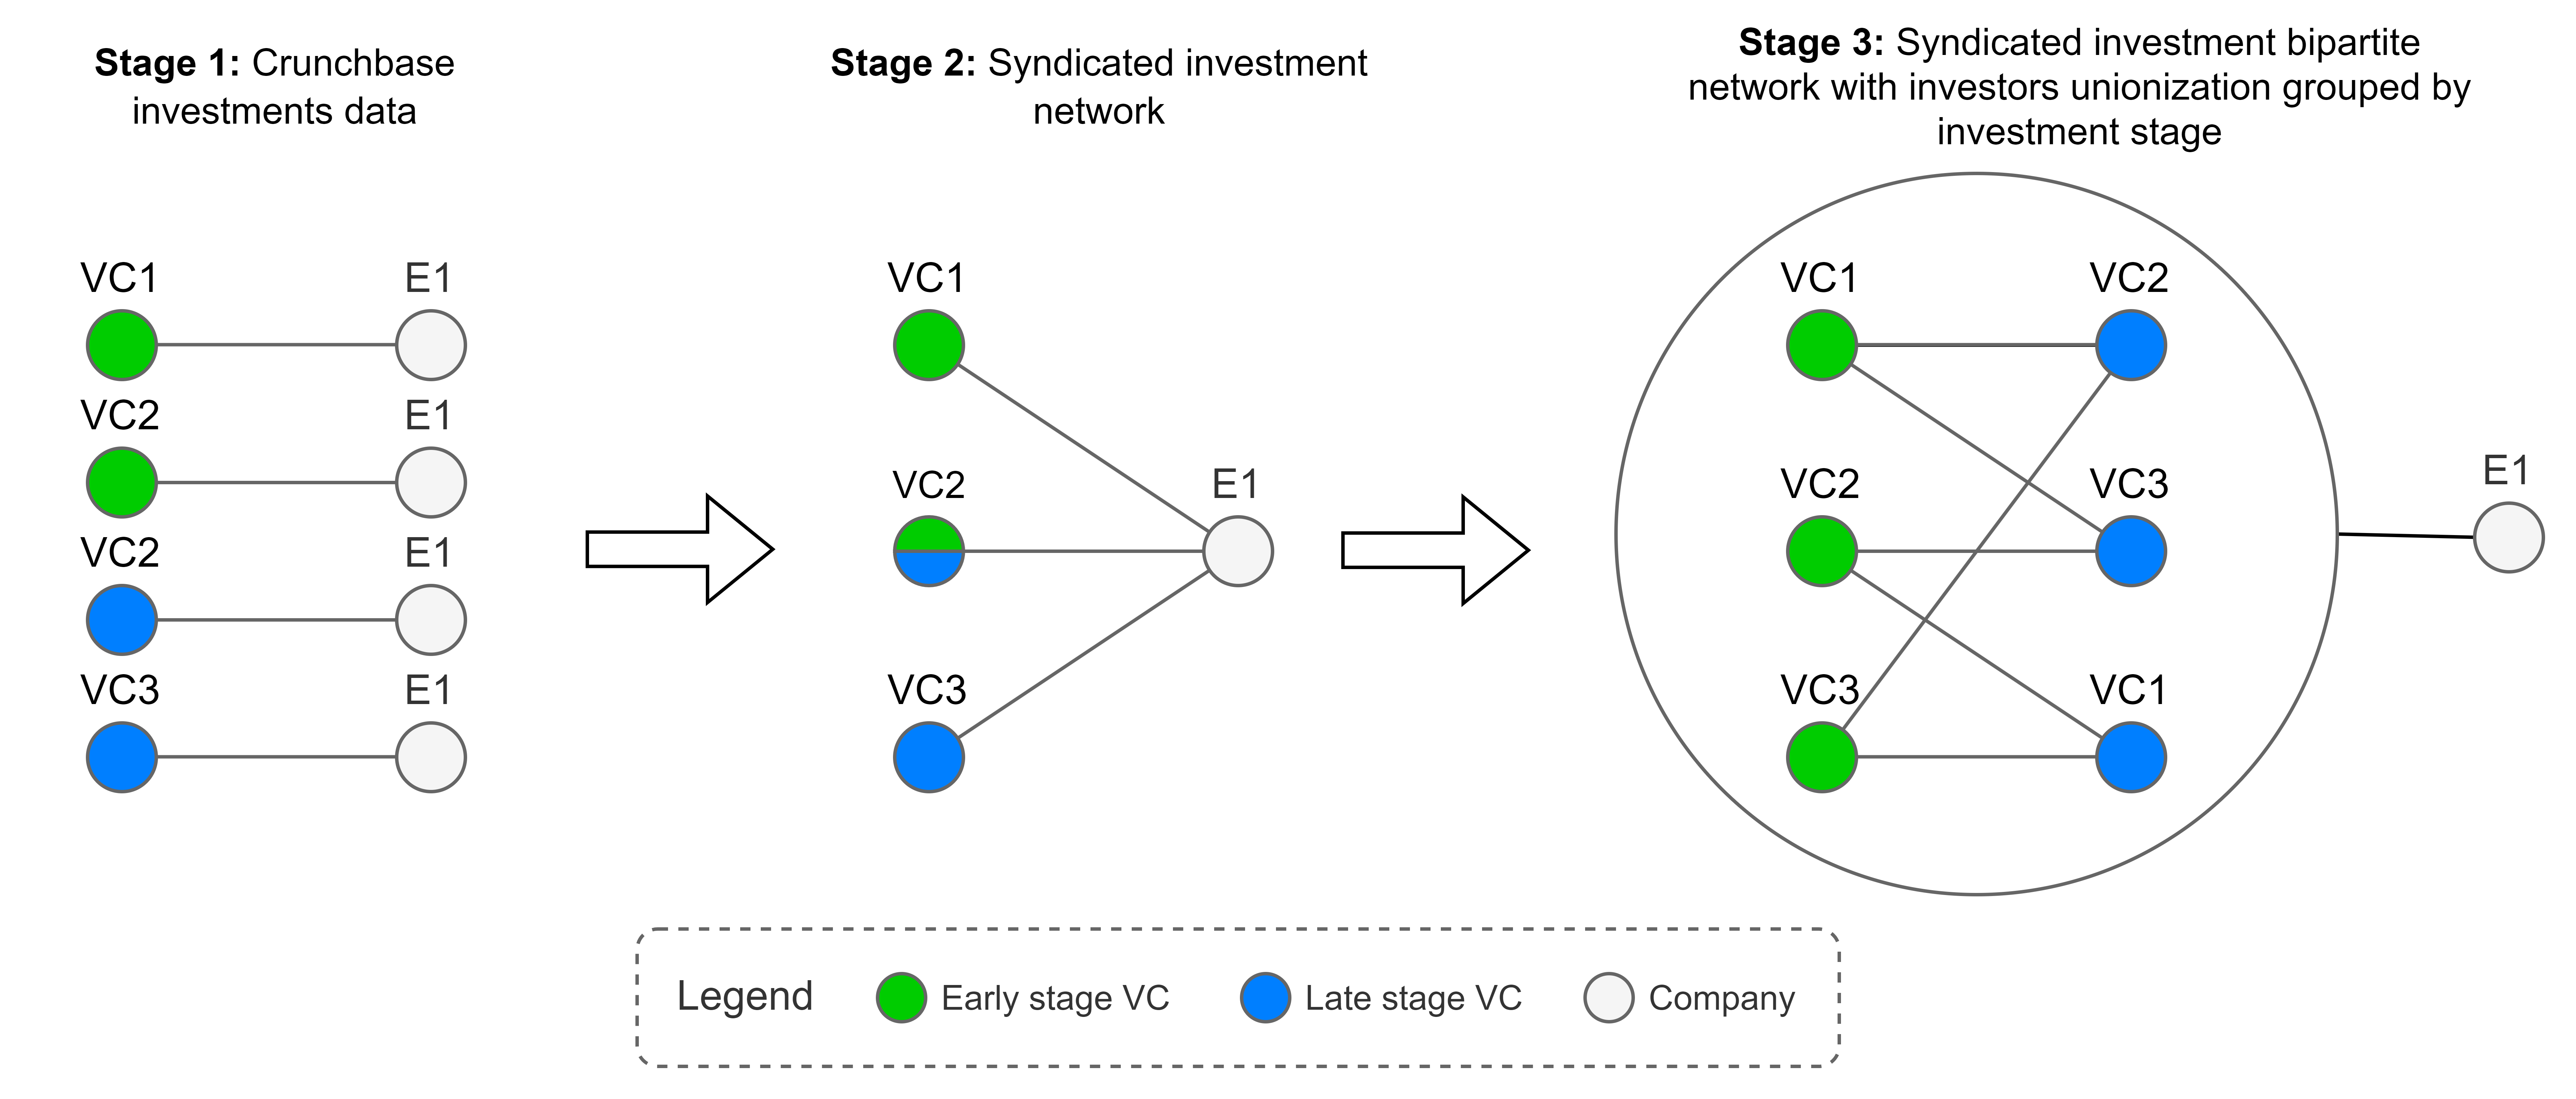
\includegraphics[width=\textwidth]{../diagrams/vc_investment_bipartite_pipeline.png}
    \caption{From event-type investment ties to bipartite syndicate networks: structuring vc relations through flow and bond models}
    \label{fig:bipartite_pipeline}
\end{figure}

\textbf{Stage 1 - Raw event-type investment ties:}
The initial Crunchbase dataset records discrete transactional relationships between venture capital firms and portfolio companies. These event-type ties represent what \cite{Borgatti2011} characterize as nominalist network constructions, where investment transactions ere defined as the fundamental tie type that constitutes the network in that stage. Each investment event creates a direct dyadic relationship between a venture capital firm and a company, but these isolated ties do not yet reveal the broader structural patterns of co-investment behavior.

\textbf{Stage 2 - Syndicated investment network construction:}
The raw event data are aggregated to identify co-investment relationships, where multiple venture capital firms participate in the same funding round or invest in the same company across different rounds. This aggregation transforms discrete investment events into a network structure where venture capital firms become indirectly connected through their shared ties to portfolio companies. Following \cite{Borgatti2011}, this step creates pathways between actors that enable analysis of their relative positions, including measures of centrality and brokerage within the investment ecosystem.

\textbf{Stage 3 - Bipartite network segmentation by investment stage:}
The final transformation reorganizes the syndicated network into a bipartite structure that separates investors based on their participation in different funding stages. 

First, investment stages are categorized into two main groups:
\begin{itemize}
    \item Early stages: angel, pre-seed, seed, and Series A
    \item Late stages: Series B through Series I
\end{itemize}

This bipartite structure reflects both flow and bond models as described by \cite{Borgatti2011}. The flow model perspective enables analysis of how resources and information traverse across investment stages, capturing the sequential nature of venture capital financing. Simultaneously, the bond model perspective recognizes that co-investors within each stage can be conceptualized as forming coordinated coalitions, reflecting solidarity ties among investors.

An important consideration in this construction involves investors who participate in both early and late stages (for example, a venture capital firm that invests in both Series A and Series C rounds). In such exceptional cases, the same investor appears as distinct agents on both sides of the bipartite network. This separation is achieved by appending the investment stage identifier to the unique investor UUID during the network construction process, effectively creating stage-specific identities for multi-stage investors. This approach ensures that the bipartite structure remains mathematically valid while preserving the analytical ability to study how the same investor behaves differently across investment stages.

The resulting bipartite graph connects two distinct sets of investors: those participating in early-stage rounds and those participating in late-stage rounds. Edges represent co-investment relationships where early-stage and late-stage investors have both invested in the same company, creating a bridge between different phases of the venture capital investment cycle.

Formally, the bipartite graph $G = (U \cup V, E)$ consists of:
\begin{align}
U &= \{u_1, u_2, \ldots, u_m\} \text{ (late-stage VCs)} \\
V &= \{v_1, v_2, \ldots, v_n\} \text{ (early-stage VCs)} \\
E &\subseteq U \times V \text{ (co-investment relationships)}
\end{align}

To prevent spurious connections from related entities, investor pairs where the first five characters of their names match are filtered out, reducing the likelihood of including different funds from the same parent organization. Furthermore, investors that participated in both early and late stages receive a suffix so they can be treated as distinct agents for each phase.

\subsection{Community Detection}

Community structure in the bipartite network is identified using modularity-based optimization methods, building on foundational work by \cite{Newman2006} who established modularity as a key metric for community detection in complex networks. For bipartite networks specifically, we employ the greedy modularity optimization algorithm following \cite{Barber2007}, who introduced a modularity definition tailored for bipartite graphs and developed corresponding algorithms that account for the distinct node sets characteristic of bipartite structures.

The choice of greedy optimization is motivated by its computational efficiency and scalability, as demonstrated by \cite{Blondel2008} in their widely-adopted Louvain algorithm. This approach iteratively merges communities to maximize the modularity score, which measures the density of connections within communities compared to connections between communities.

For a bipartite network, modularity $Q$ is defined as:
\begin{equation}
Q = \frac{1}{2m} \sum_{i,j} \left[ A_{ij} - \frac{k_i k_j}{2m} \right] \delta(c_i, c_j)
\end{equation}

where $A_{ij}$ is the adjacency matrix, $k_i$ is the degree of node $i$, $m$ is the total number of edges, $c_i$ is the community of node $i$, and $\delta(c_i, c_j)$ is 1 if nodes $i$ and $j$ are in the same community, 0 otherwise.

This methodology has proven particularly effective in venture capital research, as demonstrated by \cite{Bubna2020} who used computational methods over three decades of syndication data to identify venture capital communities. Their work establishes empirical precedent for applying community detection algorithms to co-investment networks, showing that such methods can reveal meaningful structural patterns in the investment ecosystem that may not be apparent from individual investment decisions.

\subsection{Nestedness Analysis}

Nestedness is a structural property commonly observed in ecological networks \cite{AlmeidaNeto2008} that describes the tendency for specialists to interact with a subset of the partners of generalists. In the context of venture capital networks, nestedness would indicate that investors with fewer connections tend to co-invest with a subset of the partners of more connected investors.

We measure nestedness using the NODF (Nestedness based on Overlap and Decreasing Fill) metric \cite{AlmeidaNeto2008}, which has become a standard measure for quantifying nested patterns in bipartite networks. The NODF metric is particularly well-suited for network analysis as it provides a standardized measure that accounts for both the overlap of connections and the degree differences between nodes \cite{Dormann2009}.

For a bipartite adjacency matrix $M$ with rows and columns sorted by decreasing degree, NODF is calculated as:

\begin{equation}
NODF = \frac{NODF_{rows} + NODF_{columns}}{2}
\end{equation}

where:
\begin{align}
NODF_{rows} &= \frac{100}{R(R-1)/2} \sum_{i=1}^{R-1} \sum_{j=i+1}^{R} \frac{|N_i \cap N_j|}{k_j} \text{ if } k_i > k_j \\
NODF_{columns} &= \frac{100}{C(C-1)/2} \sum_{i=1}^{C-1} \sum_{j=i+1}^{C} \frac{|N_i \cap N_j|}{k_j} \text{ if } k_i > k_j
\end{align}

Here, $R$ and $C$ are the number of rows and columns, $N_i$ represents the set of connections for node $i$, and $k_i$ is the degree of node $i$.

Using this method, NODF values range between 0 and 1 (perfect nestedness).

\subsection{Statistical Significance Testing}

To determine whether observed nestedness values differ significantly from what would be expected by chance, we employ a null model approach using the Curveball algorithm \cite{Strona2014}. This algorithm generates randomized matrices that preserve the degree sequence of both node sets while randomizing the connection patterns, representing a "hard" constraint null model that maintains structural properties while randomizing interaction patterns \cite{Dormann2009}.

The choice of degree-preserving null models is critical for nestedness interpretation, as the degree sequence itself can influence apparent nestedness patterns. By preserving degree sequences, we ensure that observed nestedness reflects genuine structural organization rather than mere consequences of heterogeneous node connectivity.

For each community, we generate 100 null matrices using 10,000 Curveball iterations. The statistical significance is assessed by comparing the observed NODF score against the distribution of null model scores:

\todo[inline]{Generate 1000 null matrices instead}

The standardized Z-score is calculated to quantify how many standard deviations the observed nestedness differs from the null expectation:

\begin{equation}
Z = \frac{NODF_{observed} - \mu_{null}}{\sigma_{null}}
\end{equation}

where $\mu_{null}$ and $\sigma_{null}$ are the mean and standard deviation of the null distribution, respectively.

The p-value is calculated empirically from the null distribution as the proportion of randomized matrices that exhibit nestedness equal to or greater than the observed value:

\begin{equation}
p = \frac{1 + \sum_{i=1}^{N} I(NODF_{null,i} \geq NODF_{observed})}{N + 1}
\end{equation}

where $N$ is the number of null matrices (100 in our case), $NODF_{null,i}$ is the nestedness score of the $i$-th null matrix, and $I(\cdot)$ is an indicator function that equals 1 when the condition is true and 0 otherwise. The addition of 1 in both numerator and denominator provides a conservative estimate that avoids p-values of exactly zero.

The p-value represents the probability of observing nestedness as high as or higher than the observed value under the null hypothesis of random co-investment patterns. Communities with $p < 0.05$ are considered to have significantly high nestedness (when observed values exceed null expectations) or significantly low nestedness (when observed values fall below null expectations), indicating that the observed nested structure is unlikely to have arisen by chance alone.

While both Z-scores and p-values assess statistical significance, they provide complementary information: the Z-score quantifies the magnitude of deviation from the null expectation in standardized units, while the p-value provides the probability of observing such deviation under the null hypothesis. In our analysis, we primarily rely on p-values for significance testing as they directly quantify the statistical evidence against the null hypothesis of random network structure.

\pagebreak

\section{Results}

\subsection{Network Characteristics}

\newcommand{\numCompanies}{22,527}
\newcommand{\numInvestors}{38,843}
\newcommand{\numInvestments}{147,832}
\newcommand{\numFundingRounds}{268,283}

The Crunchbase dataset, following the cleaning processes described in the "Methodology" section, yields \numInvestments{} investment registers, representing transactions among \numCompanies{} companies and \numInvestors{} investors.

% across \numFundingRounds{} funding rounds.

\newcommand{\numVCInvestments}{104,618}
\newcommand{\numCompaniesWithVCFund}{16,932}

Exclusion of non-venture capital investors reduces the dataset to \numVCInvestments{} investment records and \numCompaniesWithVCFund{} unique companies with venture capital funding.

\newcommand{\invPairs}{169,679}
\newcommand{\invPairsUniqueStartups}{3,666}

The division of venture capital firms into early-stage and late-stage investor groups results in \invPairs{} investment pairs comprising \invPairsUniqueStartups{} unique startups.

\todo[inline]{Add network visualization showing bipartite structure}

\newcommand{\numCommunities}{175}
\newcommand{\numTopCommunities}{5}
\newcommand{\numCommunitiesThreshold}{150}

\subsection{Community Structure and Size Distribution}

Community detection using greedy modularity optimization identifies \numCommunities{} distinct communities, with the largest communities containing over 4000 investors each, followed by 1 community with almost 1000 agents, 4 communities with more than 100 agents, and then several smaller groups.

Analysis focuses on communities with at least \numCommunitiesThreshold{} nodes to ensure statistical power for nestedness analysis. Such a threshold yields \numTopCommunities{} communities.

Table \ref{tab:community_sizes} shows the size distribution of the largest communities identified by the modularity optimization algorithm.

\todo[inline]{Rationale of threshold}

\begin{table}[htbp]
\centering
\begin{tabular}{|c|c|}
\hline
\textbf{Community ID} & \textbf{Number of Pairs} \\
\hline
0 & 4,248 \\
1 & 4,089 \\
2 & 3,959 \\
3 & 979 \\
4 & 188 \\
5 & 155 \\
6 & 137 \\
7 & 122 \\
\hline
\end{tabular}
\caption{Size distribution of the largest investor communities identified through greedy modularity optimization}
\label{tab:community_sizes}
\end{table}

The largest three communities (0, 1, and 2) contain over 12,000 investors combined, representing approximately 75\% of all investors in the network. This concentration suggests a highly centralized structure within the venture capital ecosystem, with most investment activity occurring within a small number of large communities. 

\todo[inline]{Mention literature, as this phenomena is somehow well-known}

% The community size distribution follows a typical power-law pattern observed in many social networks, where the top \numTopCommunities{} communities by size account for the majority of investors in the network, suggesting a hierarchical organization within the venture capital ecosystem.

\todo[inline]{Add figure of community size distribution}

\subsection{Nestedness Findings}

\newcommand{\numCommAnalysedNestedness}{5}

Nestedness analysis across investor communities reveals heterogeneous structural patterns. Among the \numCommAnalysedNestedness{} communities examined, one exhibits statistically significant nestedness (p < 0.01) relative to degree-preserving null models generated through the Curveball algorithm.

Figure \ref{fig:nestedness_comparison} presents the comparison between observed and null model nestedness scores, where each data point represents a distinct community positioned according to its observed NODF value against the corresponding null model mean.

\begin{figure}[htbp]
\centering
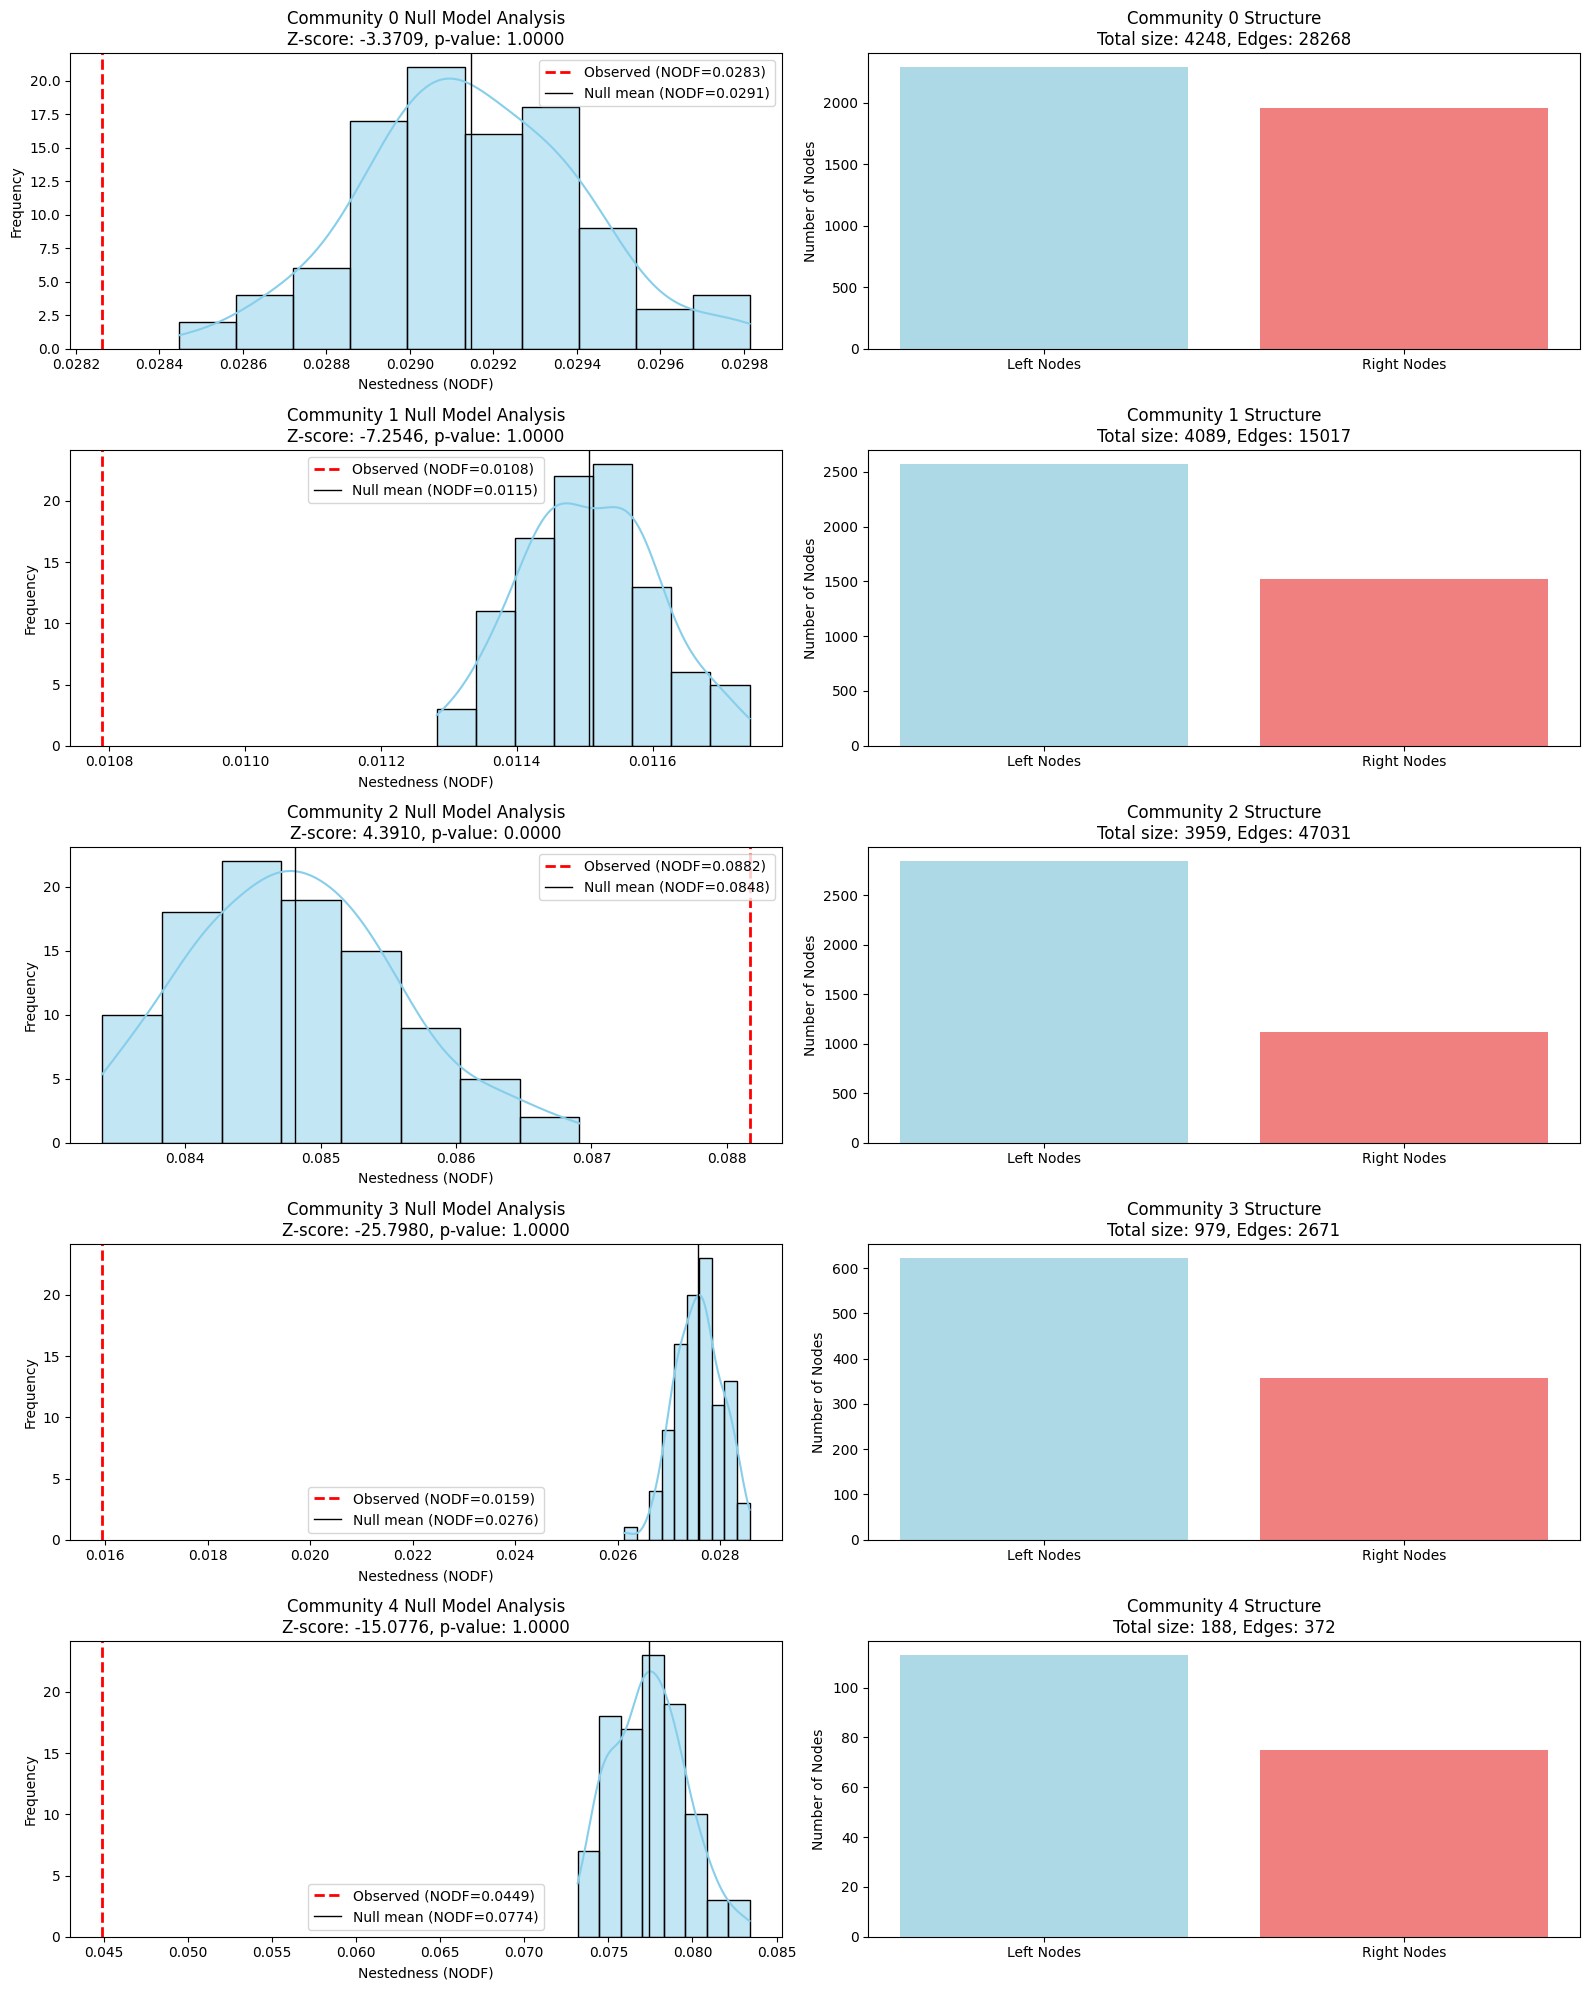
\includegraphics[width=0.8\textwidth]{./assets/null-model-analysis-top-5.png}
\caption{Comparison of observed versus null model nestedness scores for the five largest investor communities. The diagonal line represents equal observed and expected values, with points above the line indicating higher-than-random nestedness. "Left" stands for late stage investors, and "Right" for early stage ones.}
\label{fig:nestedness_comparison}
\end{figure}

\newcommand{\interestingCommunity}{2}
\newcommand{\interestingCommunityNODF}{0.088}
\newcommand{\interestingCommunityPValue}{0.00001}

Community \interestingCommunity{} demonstrates the most pronounced nestedness, exhibiting an NODF score of \interestingCommunityNODF{} with statistical significance of p = \interestingCommunityPValue{}. This hierarchical structure indicates that less-connected investors maintain co-investment relationships with subsets of partners associated with highly-connected investors, creating a hierarchical investment pattern.

Additionally, Community \interestingCommunity{} exhibits an asymmetric composition with a pronounced ratio favoring late-stage investors over early-stage investors. This imbalance contributes to the nested structure by creating hierarchical dependencies between investor types.

The following sections provide detailed characterization of this nested community through comparison with Communities 0 and 1, which serve as contrasting examples of similar-sized but differently structured investor networks.

\subsection{Communities Characterization}

Community boundaries are defined at the node level, meaning each investor belongs to exactly one community. However, edges (investment relationships) can span community boundaries when investors from different communities co-invest in the same startup.

To analyze investment patterns, we classify each syndicated investment as either: (1) intra-community if all participating investors belong to the same community, or (2) cross-community if investors from multiple communities participate together.

Table \ref{tab:investment_distribution} presents the resulting investment distribution across communities.

\begin{table}[htbp]
\centering
\begin{tabular}{|c|c|c|}
\hline
\textbf{Community} & \textbf{Number of Investments} & \textbf{Relative Proportion} \\
\hline
Community 0 & 32,164 & 19.4\% \\
Community 1 & 17,301 & 10.4\% \\
Community 2 & 55,863 & 33.6\% \\
Community 3 & 2,904 & 1.7\% \\
Cross-community & 58,329 & 35.1\% \\
\hline
\textbf{Total} & \textbf{166,561} & \textbf{100\%} \\
\hline
\end{tabular}
\caption{Distribution of syndicated investments across investor communities}
\label{tab:investment_distribution}
\end{table}

The analysis reveals important patterns in investment activity distribution. Community 2, which exhibits significant nestedness, accounts for the largest share of investments (33.6\%), containing approximately 50\% more investments than Community 0 and over three times more than Community 1. This concentration of investment activity within the nested community suggests that hierarchical investor structures may facilitate higher transaction volumes. Notably, cross-community investments represent over one-third of all transactions, indicating substantial interconnectedness across community boundaries.

\subsubsection{Funding Characteristics}

Analysis of funding patterns reveals that the nested Community 2 exhibits substantially higher funding frequency and larger investment amounts compared to the other communities, as demonstrated in Figure \ref{fig:funding_characteristics}.

\todo{Add attachment with statistical proofs}

\begin{figure}[htbp]
\centering
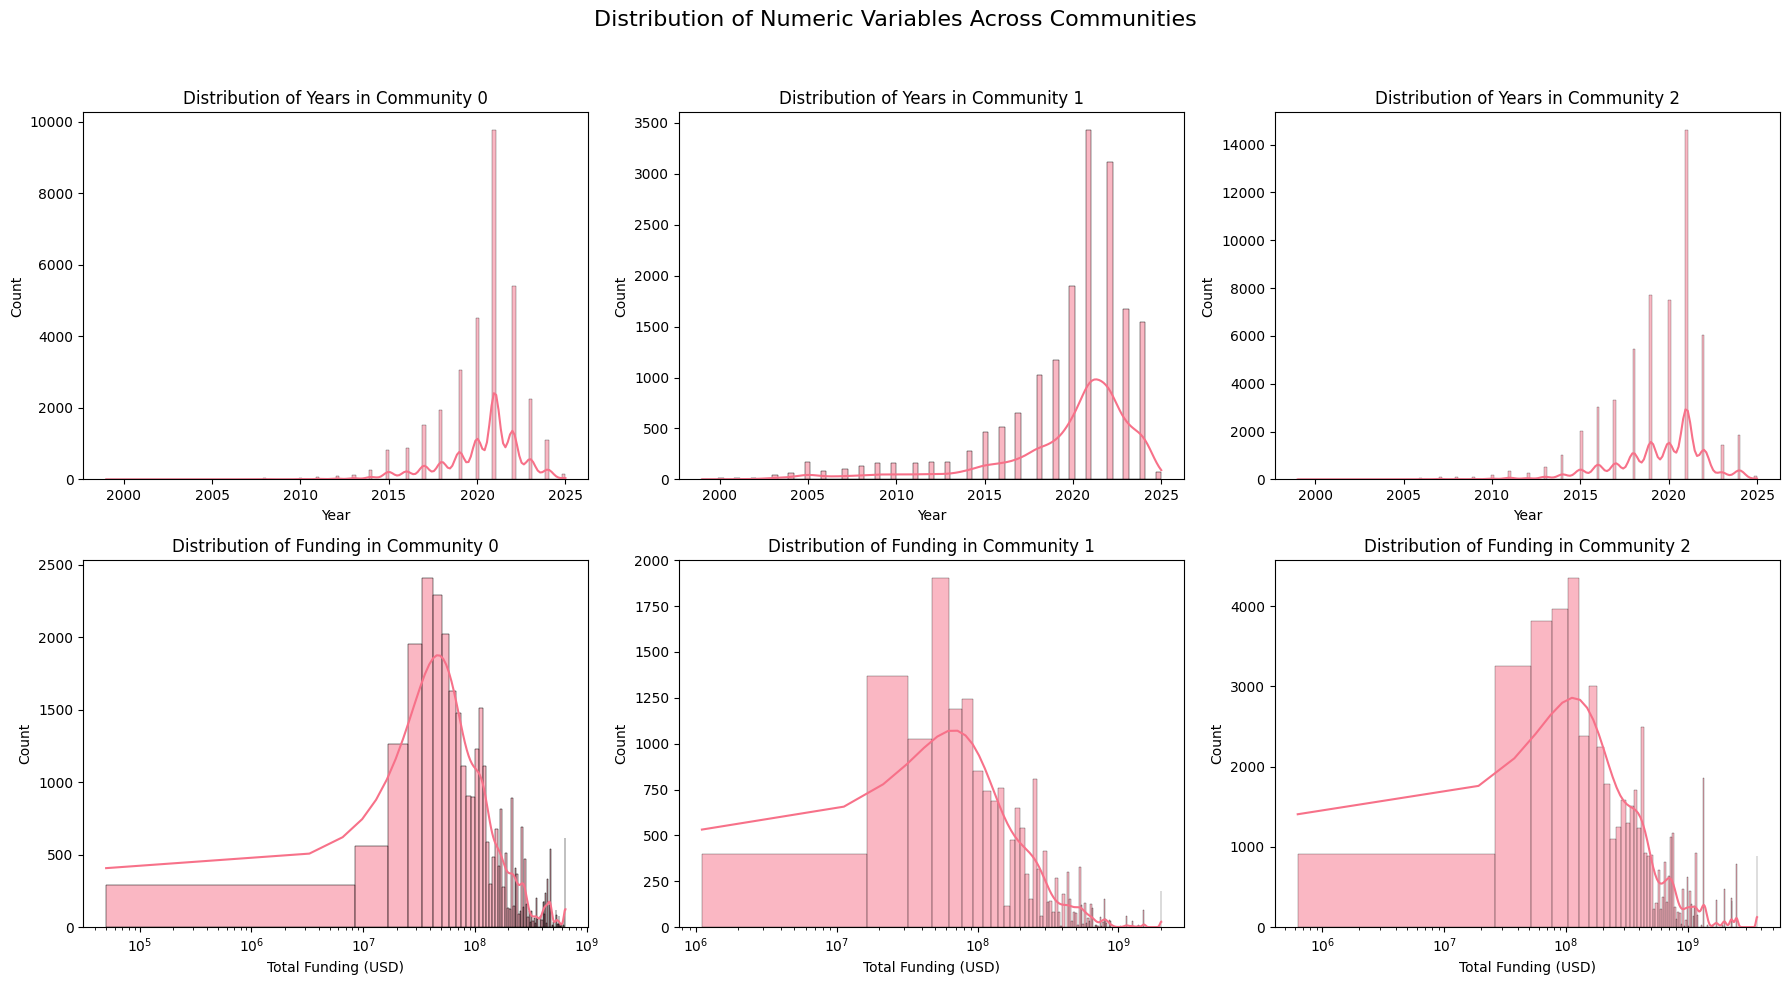
\includegraphics[width=0.8\textwidth]{./assets/funding-characteristics.png}
\caption{Funding characteristics across the three largest investor communities. The analysis reveals systematic differences in investment amounts, round frequency, and funding patterns between communities, with nested structures exhibiting distinct capital deployment strategies compared to randomly organized investor groups.}
\label{fig:funding_characteristics}
\end{figure}

\todo[]{plot a graph of distribtuion of invesments among degrees of investors}

The funding characteristics analysis indicates that nested communities exhibit concentrated capital deployment patterns, with higher-degree investors participating in larger funding rounds while maintaining broader portfolio diversification. This suggests that hierarchical investor organization may create more efficient capital allocation mechanisms compared to randomly structured networks.

Despite superficial similarities between Communities 0 and 2 in terms of size and geographic concentration within the United States, the nested structure in Community 2 appears to confer distinctive advantages. While both communities share comparable scales and American investor bases, Community 2's hierarchical organization enables it to achieve substantially higher transaction volumes (33.6\% vs. 19.4\% of total investments) and more comprehensive funding coverage across all investment stages. This pattern may suggest that nestedness functions as an organizational catalyst, transforming communities with otherwise similar characteristics into more efficient capital deployment networks.

\todo[]{add literature base for this strong assumption}

\subsubsection{Geographic Distribution}

Geographic analysis reveals distinct spatial clustering patterns across the three largest communities. Figure \ref{fig:geographic_distribution} illustrates the asymmetric geographic distributions between early-stage and late-stage investment networks.

\todo[inline]{Better format geographic distribution figure}

\begin{figure}[htbp]
\centering
\begin{subfigure}{0.48\textwidth}
    \centering
    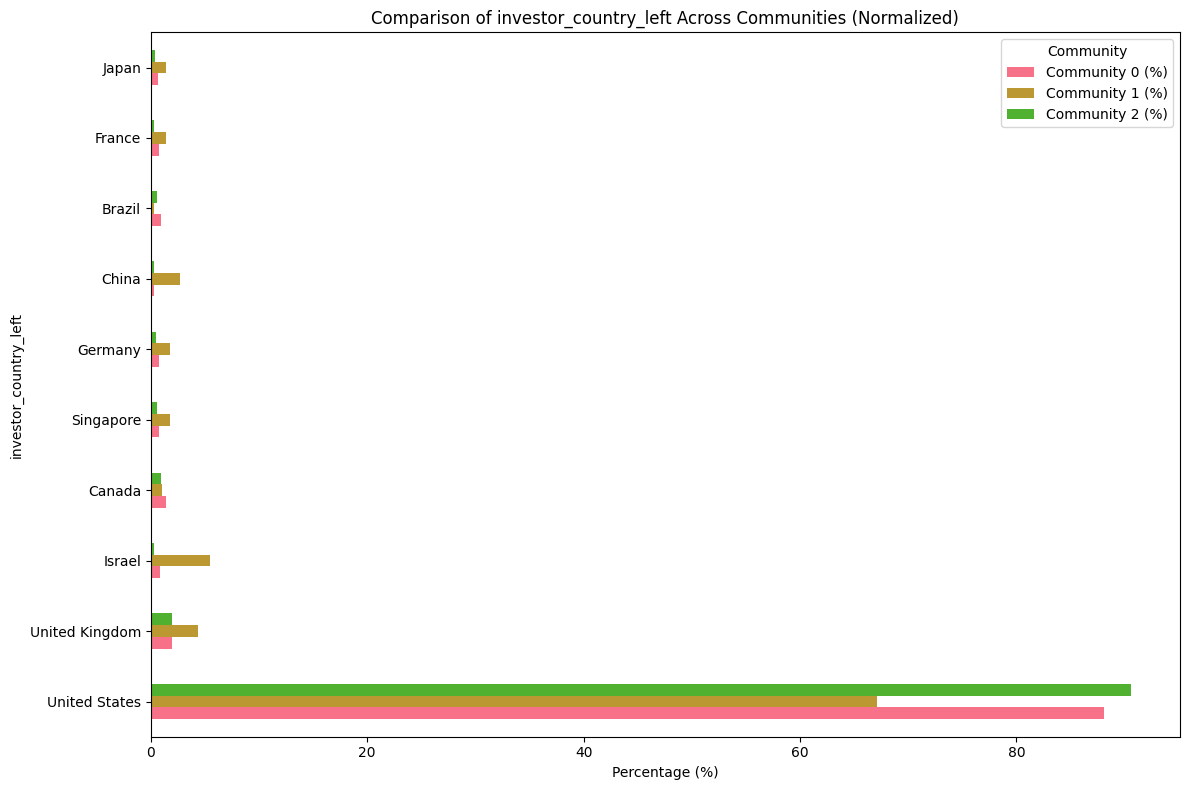
\includegraphics[width=\textwidth]{./assets/investor-left-countries.png}
    \caption{Late-stage investors geographic distribution}
    \label{fig:late_stage_geo}
\end{subfigure}
\hfill
\begin{subfigure}{0.48\textwidth}
    \centering
    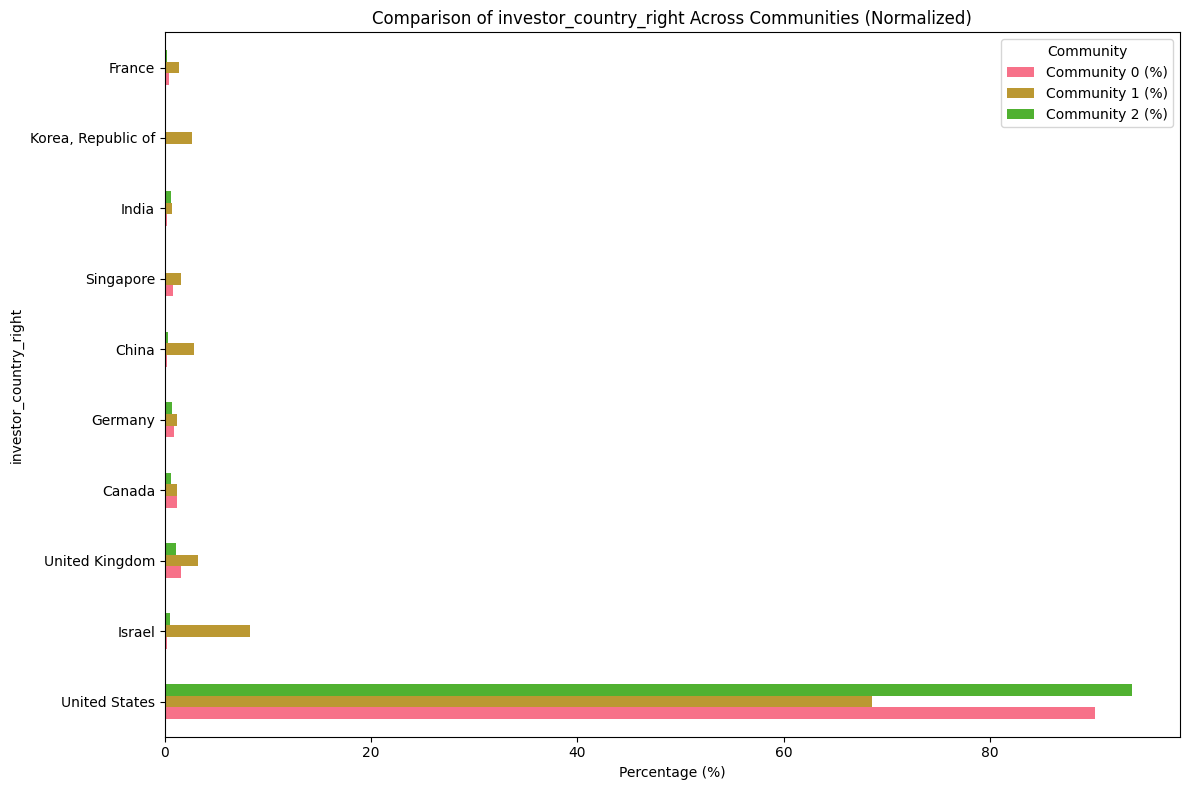
\includegraphics[width=\textwidth]{./assets/investor-right-countries.png}
    \caption{Early-stage investors geographic distribution}
    \label{fig:early_stage_geo}
\end{subfigure}
\caption{Geographic distribution of venture capital investors across the largest communities. The bipartite structure reveals differential geographic clustering between late-stage (left) and early-stage (right) investor networks, with Community 1 exhibiting greater international diversification compared to the U.S.-concentrated Communities 0 and 2.}
\label{fig:geographic_distribution}
\end{figure}

% The geographic distributions exhibit notable asymmetries: late-stage investors demonstrate greater international representation, while early-stage investors show concentrated domestic clustering. This pattern suggests stage-specific geographic preferences that may reflect risk tolerance, regulatory constraints, or information asymmetries across international markets.

Communities 0 and 2 exhibit similar geographic profiles with predominantly American investors, reflecting the dominance of U.S.-based venture capital (important to remember our dataset contains only American startups' investments, which include international investors). However, regional analysis within the United States reveals a striking pattern: Community 2 demonstrates exceptional concentration in California, particularly Silicon Valley, with approximately 50\% more California-based investors than either Community 0 or Community 1 for both late-stage and early-stage investor categories.

This Silicon Valley concentration in the nested Community 2 is particularly significant given the region's status as the world's premier innovation ecosystem. The dominance of California investors in the only statistically nested community suggests a potential relationship between geographic clustering in innovation hubs and the emergence of hierarchical investment structures. This pattern may reflect the dense information networks, frequent face-to-face interactions, and shared risk assessment practices characteristic of Silicon Valley's venture capital community.

In contrast, Community 1 demonstrates significantly greater international diversification, with substantial representation from Israel, the United Kingdom, China, South Korea, Singapore, and France. This international composition in Community 1 may reflect different risk tolerance profiles, regulatory environments, or access to cross-border deal flow compared to the more domestically concentrated communities.

\subsubsection{Investment Stage Preferences}

The investment stage distributions reveal systematic specialization patterns across communities that align with their geographic profiles and transaction volumes. Figure \ref{fig:investment_stage_distribution} demonstrates the distribution patterns of investment types within the bipartite network structure.

\begin{figure}[htbp]
\centering
\begin{subfigure}{0.48\textwidth}
    \centering
    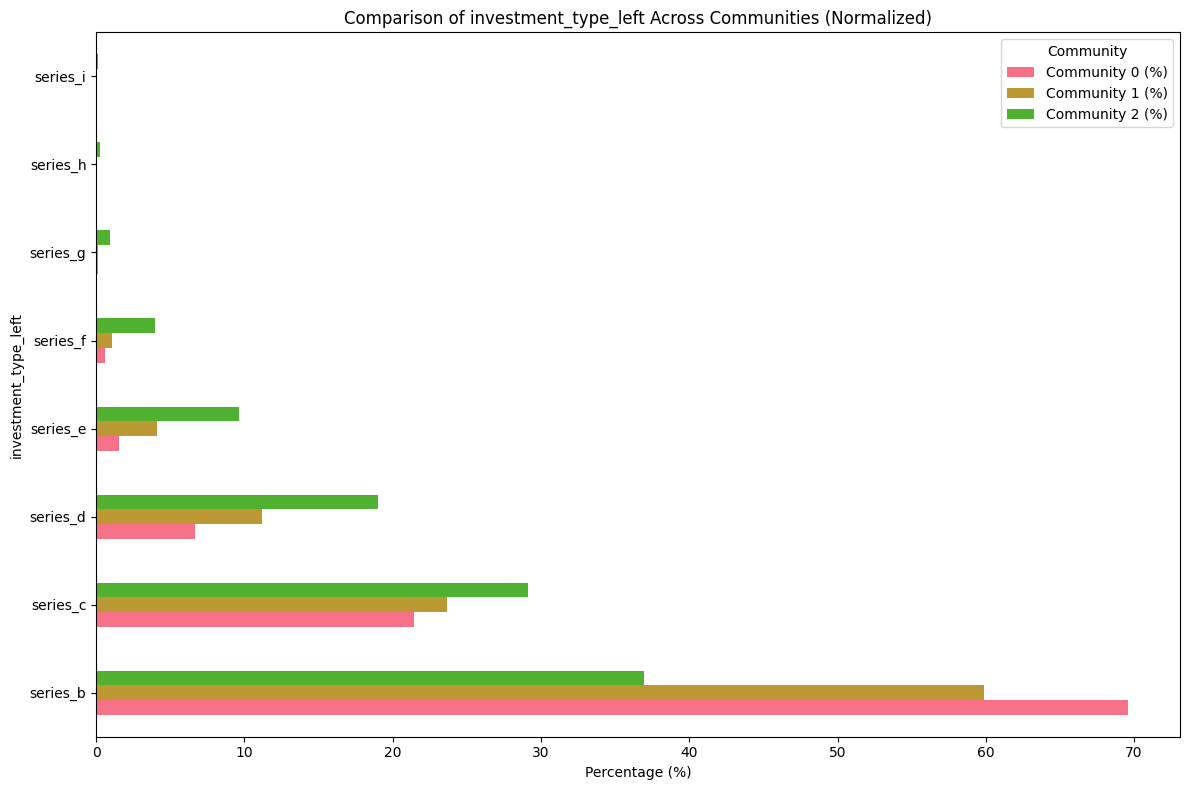
\includegraphics[width=\textwidth]{./assets/late-investment-types-distribution.png}
    \caption{Late-stage investment types distribution}
    \label{fig:late_stage_types}
\end{subfigure}
\hfill
\begin{subfigure}{0.48\textwidth}
    \centering
    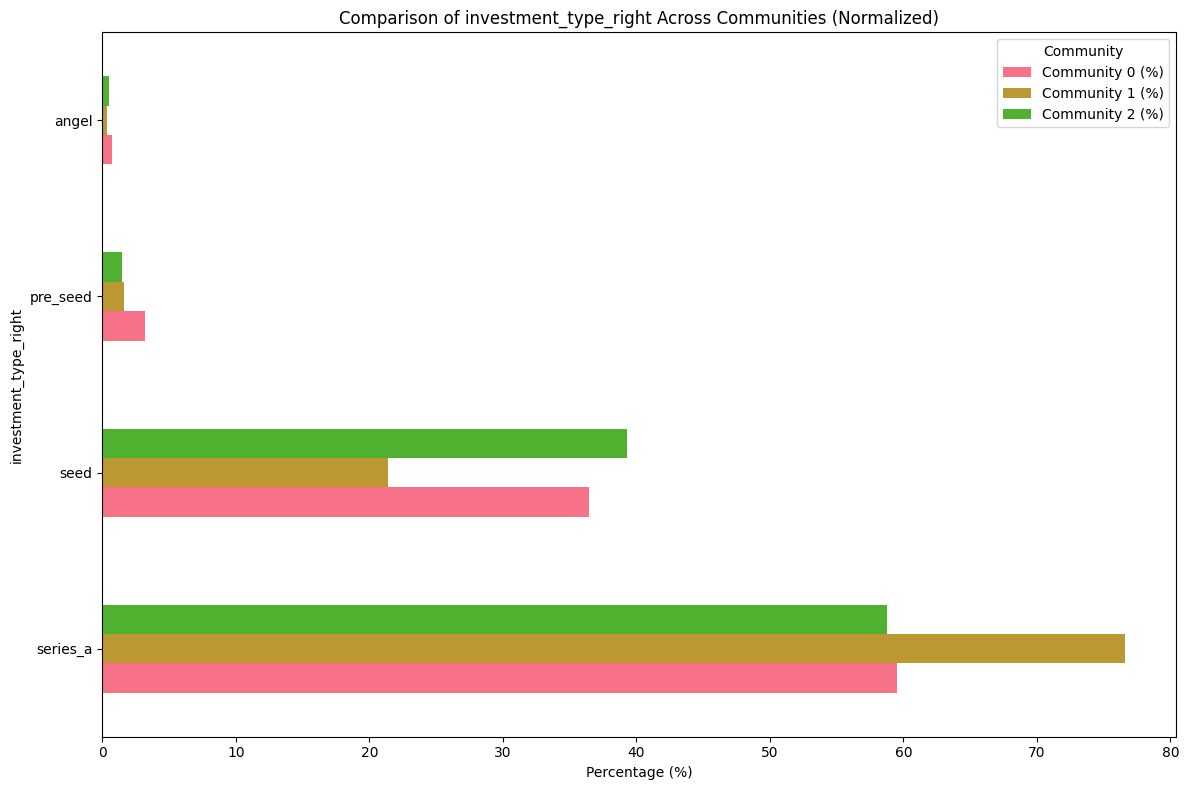
\includegraphics[width=\textwidth]{./assets/early-investment-types-distribution.png}
    \caption{Early-stage investment types distribution}
    \label{fig:early_stage_types}
\end{subfigure}
\caption{Investment stage distribution across the three largest communities. The distribution patterns reveal stage-specific specialization within investor communities.}
\label{fig:investment_stage_distribution}
\end{figure}


\todo[inline]{Comment investment stages distribution}

\textbf{Late-stage investment patterns:} Community 2 dominates Series C and later funding rounds, demonstrating its role in growth-stage capital deployment. Community 1, despite its smaller transaction volume, shows strong representation in Series B and later stages, with participation rates exceeding Community 0 in Series C and beyond. Community 0 exhibits particular strength in Series B rounds while maintaining lower participation in later stages compared to Community 2.

\textbf{Early-stage investment patterns:} Community 2 shows prominence in seed-stage investments while maintaining comparable levels to Community 0 in Series A funding. Both Communities 0 and 2 participate actively in angel and seed rounds, though Community 0 shows relatively higher pre-seed activity. Community 1 demonstrates concentrated focus on Series A investments, aligning with its international profile and suggesting specialization in cross-border early-growth funding.

These stage-specific patterns suggest that the nested structure in Community 2 facilitates participation across the entire funding spectrum, from seed to late-stage rounds, potentially enabling more comprehensive support for portfolio companies throughout their development lifecycle.

\subsubsection{Sectoral Focus}

The sectoral analysis reveals distinct specialization patterns that align with each community's structural and geographic characteristics. Figure \ref{fig:sectoral_distribution} illustrates the distribution of investment focus across technology sectors, demonstrating how different communities exhibit varying degrees of sectoral concentration.

\begin{figure}[htbp]
\centering
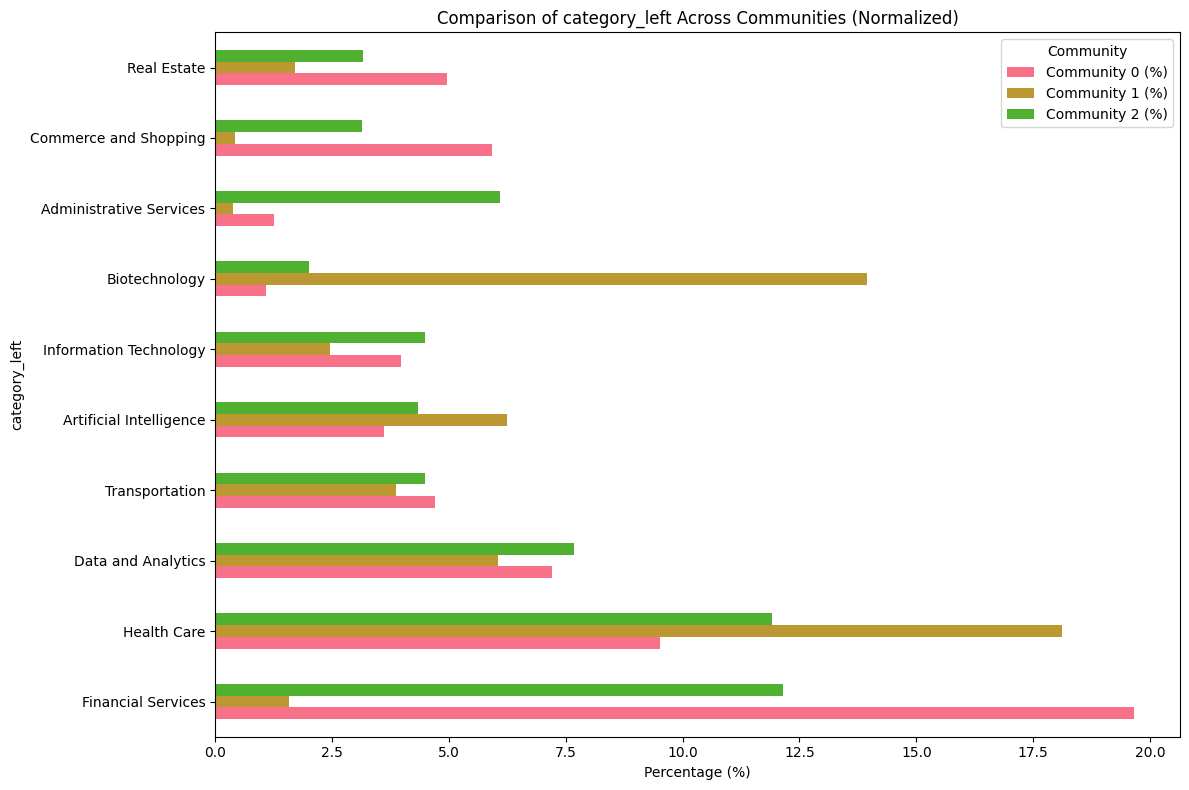
\includegraphics[width=0.8\textwidth]{./assets/sectorial-distribution.png}
\caption{Sectoral distribution across the three largest investor communities. The analysis reveals differential industry focus patterns, with certain communities demonstrating concentrated investment strategies in specific technology sectors while others maintain broader sectoral diversification.}
\label{fig:sectoral_distribution}
\end{figure}

\todo[inline]{Comment sectorial distribution}

\textbf{Community 0:} Concentrates in real estate, commerce and shopping, and financial services, while maintaining standard representation in information technology and artificial intelligence. Notably absent from administrative services and biotechnology, suggesting specialized expertise in consumer-facing and financial technology sectors.

\textbf{Community 1:} Specializes significantly in biotechnology and healthcare, with enhanced artificial intelligence focus compared to other communities. Shows reduced interest in real estate, commerce and shopping, and administrative services. The biotechnology concentration aligns with its international composition, potentially reflecting access to global biotech innovation hubs.

**Community 2:** The nested community exhibits strong representation in administrative services while maintaining comparable levels to Community 0 in information technology and artificial intelligence. Despite its larger transaction volume, it shows lower concentration in real estate and financial services than Community 0, suggesting that nested structure facilitates broader sectoral participation rather than concentrated specialization. This sectoral breadth, combined with the community's Silicon Valley concentration, indicates that nestedness may enable more diversified investment strategies within innovation-rich geographic clusters.

Community 0 serves as an effective structural baseline for comparison with nested Community 2, given their similar geographic profiles and certain sectoral overlaps, while differing significantly in network organization and transaction volumes. The systematic differences observed between these structurally similar communities underscore a potential impact of nested organization on investment behavior and capital deployment efficiency.

\todo[inline]{Add overall comparison}
\todo[inline]{Comment more on funding characteristics}



\section{Discussion and Implications}

The discovery of significantly nested communities within the venture capital network provides new insights into investor behavior and startup access to capital. The hierarchical structure in Community 2 suggests that informal investment hierarchies may systematically influence funding accessibility for entrepreneurs.

The concentration of nested structure specifically within Silicon Valley investors adds a critical geographic dimension to these findings. Community 2's exceptional dominance by California-based investors, particularly those in Silicon Valley, suggests that geographic clustering within the world's premier innovation ecosystem may facilitate the emergence of hierarchical investment structures. This pattern indicates that dense information networks, frequent face-to-face interactions, and shared risk assessment practices characteristic of innovation hubs may naturally give rise to nested investor relationships.

Furthermore, the comparative analysis between Communities 0 and 2 reveals that nestedness functions as an organizational catalyst that transforms otherwise similar investor communities. Despite comparable sizes and geographic concentration within the United States, Community 2's nested structure enables substantially higher transaction volumes and more comprehensive funding coverage across all investment stages. This suggests that network topology, rather than community size or geographic distribution alone, may be the critical determinant of investment ecosystem efficiency.

\subsection{Degree Distribution Patterns and Hub Organization}

The analysis of degree distributions across communities reveals fundamental organizational differences that complement the nestedness findings. All three communities exhibit power-law degree distributions characteristic of scale-free networks \cite{Borgatti2011}, but with distinct magnitude and structural parameters that reflect different organizational strategies.

The remarkable similarity in degree distribution magnitudes between Communities 0 and 2, contrasted with Community 1's consistently lower values, suggests that network scale alone does not determine investment efficiency. Community 2's superior performance in investment volumes and nested organization occurs despite degree distribution patterns nearly identical to Community 0. This finding reinforces that the specific arrangement of connections, rather than their quantity or distribution, drives the observed efficiency advantages.

Analysis of high-degree nodes (network hubs) reveals distinct organizational philosophies across communities. Community 2's hub structure demonstrates exceptional concentration among early-stage Silicon Valley investors, with SV Angel achieving remarkable connectivity across both seed and Series A stages. This pattern contrasts sharply with Community 0's more diversified hub structure and Community 1's balanced early-late stage distribution. The concentration of hubs within the early-stage investment category in Community 2 may facilitate the nested structure by creating clear hierarchical pathways from early-stage to late-stage investment relationships.

The positive correlation between degree centrality and investment activity across all communities validates network position as a predictor of investor influence. However, the strength of this relationship appears amplified within the nested Community 2, suggesting that hierarchical organization may enhance the efficiency of high-degree investors in deploying capital and identifying investment opportunities.

\subsection{Temporal Dynamics and Phase Transition Emergence}

\todo[inline]{Add observation that literature on other formations were already explored, but VC-VC is rare}

The temporal evolution analysis of Community 2 provides unprecedented insight into how nested structures emerge within VC-VC investment networks. The identification of a sharp phase transition in 2019, rather than gradual nestedness development, challenges assumptions about evolutionary network organization and suggests threshold-dependent emergence mechanisms.

The three-phase evolution pattern—non-significant period (2007-2018), transition (2019), and sustained significance (2019-2024) indicates that nested organization in venture capital networks may represent a distinct organizational state that emerges discontinuously when specific conditions are met. This finding aligns with theoretical predictions from complex network theory regarding critical transitions in topological properties \cite{Mariani2019}.

The apparent paradox of decreasing absolute nestedness scores (from 0.38 to 0.088) coinciding with increasing statistical significance reflects sophisticated changes in network organization. As the network grew substantially larger, maintaining even modest levels of hierarchical organization became increasingly difficult under random formation processes, making the observed nested patterns more statistically remarkable. This pattern suggests that the nested structure represents increasingly precise organizational control as the investment ecosystem scales.

The correspondence between nestedness emergence and specific connectance thresholds (approximately 0.026) provides practical insights for ecosystem development. This threshold may represent a critical density where hierarchical organization becomes sustainable within large-scale investment networks, offering guidance for policy interventions aimed at fostering similar organizational efficiency in other innovation ecosystems.

The asymmetric evolution of investor types—increasing late-stage participation coupled with stabilizing early-stage numbers—may have facilitated nested structure emergence by creating conditions favoring hierarchical relationships. This pattern suggests that the development of nested organization may require specific demographic conditions within investor communities, rather than simply network growth or density changes.

\subsection{Network Robustness and Resilience}

The nested structures challenge assumptions of random mixing in venture capital markets, suggesting that certain investors function as "gatekeepers" who control access to broader investment networks. This finding aligns with social network theories about structural holes and brokerage positions \cite{Borgatti2011}.

Following insights from nestedness research in complex networks \cite{Mariani2019}, the hierarchical organization observed in Community 2 may confer distinct robustness properties to the venture capital ecosystem. In mutualistic networks, nestedness typically enhances stability against random node removal but creates vulnerability to targeted elimination of highly connected nodes. Applied to venture capital, this suggests that while nested investor communities may be resilient to random investor departures, they could be particularly vulnerable to the exit of key hub investors.

The concept of "mutualistic trade-offs" from ecological network theory provides a framework for understanding these dynamics. In nested venture capital communities, less-connected investors maintain relationships with subsets of the partners associated with highly-connected investors, creating dependencies that could influence network stability. Future research should investigate whether less-connected venture capital firms exhibit higher exit probabilities, which would support the hypothesis that nestedness creates hierarchical fragility patterns.


\section{Conclusion and Future Directions}

\subsection{Individual Nestedness Contributions}

An important avenue for future research involves analyzing individual nestedness contributions within these communities. Rather than treating nestedness as a global network property, examining how specific investors contribute to the overall nested structure could reveal mechanisms driving community formation and persistence. This approach could help predict which network positions are most vulnerable to disruption and identify critical nodes whose removal would significantly alter community structure.

Understanding individual contributions to nestedness could also inform strategies for network intervention and ecosystem development. If certain investor positions disproportionately contribute to nested stability, targeted support or policy interventions could enhance overall ecosystem resilience.

\subsection{Dynamic Network Evolution}

The temporal analysis reveals several critical insights about the dynamic processes underlying venture capital network organization. The sharp phase transition observed in Community 2's nestedness evolution suggests that network topology may be subject to discontinuous organizational changes rather than gradual evolution. This finding has important implications for understanding how investment ecosystems develop and potentially collapse.

The three-phase temporal pattern—extended non-significant periods, rapid transition, and sustained significance—may represent a general framework for understanding organizational emergence in investment networks. The identification of specific connectance thresholds (approximately 0.026) associated with nestedness emergence provides quantitative targets for ecosystem development strategies. Future research should investigate whether similar threshold effects exist in other geographic markets and whether policy interventions can facilitate reaching these critical organizational states.

The asymmetric evolution of investor types during the transition period offers insights into the demographic conditions that may facilitate nested organization. The pattern of increasing late-stage investor participation coupled with stabilizing early-stage numbers suggests that hierarchical organization may require specific ratios between investor types. This finding could inform strategies for ecosystem development in emerging markets, where the balance of early-stage and late-stage capital availability is often suboptimal.

The temporal analysis also reveals that nestedness persistence appears robust once established. The sustained significance observed from 2019-2024, despite substantial network growth and changing market conditions, suggests that nested organization may represent a stable attractor state in investment network evolution. This stability has important implications for long-term ecosystem planning and suggests that successful development of nested organization may provide lasting competitive advantages for innovation hubs.

\subsection{Causal Mechanisms and Economic Outcomes}

The identification of these nested communities opens several avenues for future research into the social and economic mechanisms that drive venture capital ecosystem organization. Chapter 5 of "Nestedness in complex networks" \cite{Mariani2019} provides theoretical frameworks for understanding why nestedness emerges in complex systems, including factors such as heterogeneous node fitness, temporal constraints on link formation, and spatial or industry-specific constraints on partnership formation.

Investigating whether nested communities provide superior or inferior outcomes for portfolio companies compared to randomly organized investor groups represents a crucial research priority. The concentrated capital deployment patterns observed in Community 2 suggest potential efficiency advantages, but these must be weighed against potential risks from reduced diversity and increased systemic vulnerability.

\subsection{Policy and Ecosystem Development Implications}

Understanding these patterns may inform policy discussions about startup ecosystem development and investor network formation. The concentration of nested structures within Silicon Valley suggests that geographic proximity within innovation hubs may be a prerequisite for the emergence of hierarchical investor relationships. This finding has important implications for ecosystem development strategies in other regions seeking to replicate Silicon Valley's success.

If nested structures facilitate higher transaction volumes and more comprehensive funding support, as observed in Community 2, policies that encourage the formation of such hierarchical investor relationships might enhance ecosystem efficiency. However, the geographic specificity of this pattern suggests that simply replicating formal structures may be insufficient—the dense information networks and shared practices of established innovation hubs appear to be necessary conditions for nested organization to emerge.

Conversely, if nestedness creates barriers to entry for new investors or reduces access for certain entrepreneur populations, regulatory interventions might be warranted to promote more equitable network organization. The dominance of Silicon Valley investors in the nested community raises questions about geographic bias in capital allocation and whether hierarchical structures may inadvertently concentrate investment opportunities within established innovation centers.

The possibility of network rewiring, analogous to ecological community adaptation, might confer additional robustness to venture capital ecosystems. Policies that facilitate investor mobility and relationship reformation could enhance system-wide resilience while maintaining the efficiency benefits of nested organization.

This analysis provides the foundation for deeper investigation into how nested investor communities influence entrepreneurial ecosystems and capital allocation efficiency, which will be the focus of subsequent research phases.

\todo[inline]{Investigate whether the Silicon Valley concentration in nested communities reflects unique geographic advantages, information network density, or institutional factors that could be replicated in other innovation ecosystems.}

\todo[inline]{Examine the relationship between geographic clustering in innovation hubs and the emergence of nested investor structures across different global venture capital markets.}

\todo[inline]{Investigate the economic consequences of nested community structure on startup success rates and funding efficiency.}

\todo[inline]{Analyze individual nestedness contributions to identify critical nodes and understand how specific investor positions contribute to overall community stability and structure.}

\todo[inline]{Investigate the robustness properties of nested venture capital communities, particularly vulnerability to targeted removal of highly connected investors versus resilience to random investor departures.}

\todo[inline]{Examine the relationship between investor position within nested hierarchies and probability of network exit, testing whether less-connected VCs exhibit higher departure rates.}

\todo[inline]{Apply social network theories of structural holes to understand the role of highly connected investors in nested communities and their function as potential gatekeepers.}

\todo[inline]{Investigate whether the nested structure reflects information asymmetries, risk-sharing mechanisms, or industry-specific constraints among investors.}

\todo[inline]{Develop theoretical models to explain the emergence of nested structures in investment networks, incorporating insights from Chapter 5 of "Nestedness in complex networks" regarding heterogeneous node fitness and temporal constraints.}

\todo[inline]{Compare nestedness patterns across different geographic markets and time periods to understand generalizability and cultural influences on network organization.}

\todo[inline]{Investigate the relationship between degree distribution patterns and nestedness emergence, examining whether specific scale-free parameter ranges facilitate hierarchical organization.}

\todo[inline]{Explore the role of hub investor strategies in nested community formation, particularly investigating how early-stage hub concentration may facilitate hierarchical pathway development.}

\todo[inline]{Analyze the predictive power of connectance thresholds for nestedness emergence in other venture capital markets and innovation ecosystems.}

\todo[inline]{Examine the stability mechanisms that maintain nested organization once established, investigating whether demographic balance between investor types is necessary for persistence.}


\section{Conclusion and Future Directions}

\subsection{Individual Nestedness Contributions}

An important avenue for future research involves analyzing individual nestedness contributions within these communities. Rather than treating nestedness as a global network property, examining how specific investors contribute to the overall nested structure could reveal mechanisms driving community formation and persistence. 

This approach could help predict which network positions are most vulnerable to disruption and identify critical nodes whose removal would significantly alter community structure.

Understanding individual contributions to high nestedness could also inform strategies for network intervention and ecosystem development. If certain investor positions disproportionately contribute to highly nested stability, targeted support or policy interventions could enhance overall ecosystem resilience.

\subsection{Dynamic Network Evolution}

The temporal analysis reveals several critical insights about the dynamic processes underlying venture capital network organization. The sharp phase transition observed in Community 2's nestedness evolution suggests that network topology may be subject to discontinuous organizational changes rather than gradual evolution. This finding has important implications for understanding how investment ecosystems develop and potentially collapse.

The three-phase temporal pattern (extended periods with significantly low nestedness, rapid transition, and sustained high nestedness) may represent a general framework for understanding organizational emergence in investment networks. The identification of specific connectance thresholds (approximately 0.026) associated with the emergence of high nestedness provides quantitative targets for ecosystem development strategies. 

Future research should investigate whether similar threshold effects exist in other geographic markets and whether policy interventions can facilitate reaching these critical organizational states.

The asymmetric evolution of investor types during the transition period offers insights into the demographic conditions that may facilitate highly nested organization. The pattern of increasing late-stage investor participation coupled with stabilizing early-stage numbers suggests that hierarchical organization may require specific ratios between investor types. 

This finding could inform strategies for ecosystem development in emerging markets, where the balance of early-stage and late-stage capital availability is often suboptimal.

The temporal analysis also reveals that high nestedness persistence appears robust once established. The sustained high nestedness observed from 2019-2024, despite substantial network growth and changing market conditions, suggests that highly nested organization may represent a stable attractor state in investment network evolution. 

This stability has important implications for long-term ecosystem planning and suggests that successful development of highly nested organization may provide lasting competitive advantages for innovation hubs.

\subsection{Causal Mechanisms and Economic Outcomes}

The identification of these nested communities opens several avenues for future research into the social and economic mechanisms that drive venture capital ecosystem organization. \cite{Mariani2019} provides theoretical frameworks for understanding why nestedness emerges in complex systems, including factors such as heterogeneous node fitness, temporal constraints on link formation, and spatial or industry-specific constraints on partnership formation.

Investigating whether highly nested communities provide superior or inferior outcomes for portfolio companies compared to randomly organized investor groups represents a research opportunity. The concentrated capital deployment patterns observed in Community 2 suggest potential efficiency advantages, but these must be weighed against potential risks from reduced diversity and increased systemic vulnerability.

\subsection{Policy and Ecosystem Development Implications}

The concentration of highly nested structures within Silicon Valley suggests that geographic proximity within innovation hubs may be a prerequisite for the emergence of hierarchical investor relationships. This finding has important implications for ecosystem development strategies in other regions seeking to replicate Silicon Valley's success. 

Understanding these patterns may inform policy discussions about startup ecosystem development and investor network formation. If highly nested structures facilitate higher transaction volumes and more comprehensive funding support, as observed in Community 2, policies that encourage the formation of such hierarchical investor relationships might enhance ecosystem efficiency. 

However, the geographic specificity of this pattern suggests that simply replicating formal structures may be insufficient—the dense information networks and shared practices of established innovation hubs appear to be necessary conditions for highly nested organization to emerge.

Conversely, if high nestedness creates barriers to entry for new investors or reduces access for certain entrepreneur populations, regulatory interventions might be warranted to promote more equitable network organization. 

The dominance of Silicon Valley investors in the highly nested community raises questions about geographic bias in capital allocation and whether hierarchical structures may inadvertently concentrate investment opportunities within established innovation centers.

The possibility of network rewiring \todo[]{mention literature about rewiring}, analogous to ecological community adaptation, might confer additional robustness to venture capital ecosystems. Policies that facilitate investor mobility and relationship reformation could enhance system-wide resilience while maintaining the efficiency benefits of highly nested organization.

% This analysis provides the foundation for deeper investigation into how nested investor communities influence entrepreneurial ecosystems and capital allocation efficiency, which will be the focus of subsequent research phases.

\todo[inline]{Investigate whether the Silicon Valley concentration in nested communities reflects unique geographic advantages, information network density, or institutional factors that could be replicated in other innovation ecosystems.}

\todo[inline]{Examine the relationship between geographic clustering in innovation hubs and the emergence of nested investor structures across different global venture capital markets.}

\todo[inline]{Investigate the economic consequences of nested community structure on startup success rates and funding efficiency.}

\todo[inline]{Analyze individual nestedness contributions to identify critical nodes and understand how specific investor positions contribute to overall community stability and structure.}

\todo[inline]{Investigate the robustness properties of nested venture capital communities, particularly vulnerability to targeted removal of highly connected investors versus resilience to random investor departures.}

\todo[inline]{Examine the relationship between investor position within nested hierarchies and probability of network exit, testing whether less-connected VCs exhibit higher departure rates.}

\todo[inline]{Apply social network theories of structural holes to understand the role of highly connected investors in nested communities and their function as potential gatekeepers.}

\todo[inline]{Investigate whether the nested structure reflects information asymmetries, risk-sharing mechanisms, or industry-specific constraints among investors.}

\todo[inline]{Develop theoretical models to explain the emergence of nested structures in investment networks, incorporating insights from Chapter 5 of "Nestedness in complex networks" regarding heterogeneous node fitness and temporal constraints.}

\todo[inline]{Compare nestedness patterns across different geographic markets and time periods to understand generalizability and cultural influences on network organization.}

\todo[inline]{Investigate the relationship between degree distribution patterns and nestedness emergence, examining whether specific scale-free parameter ranges facilitate hierarchical organization.}

\todo[inline]{Explore the role of hub investor strategies in nested community formation, particularly investigating how early-stage hub concentration may facilitate hierarchical pathway development.}

\todo[inline]{Analyze the predictive power of connectance thresholds for nestedness emergence in other venture capital markets and innovation ecosystems.}

\todo[inline]{Examine the stability mechanisms that maintain nested organization once established, investigating whether demographic balance between investor types is necessary for persistence.}

\pagebreak
}

\bibliographystyle{plain}
\bibliography{references}

\end{document}
